\section{Estado del arte}
\subsection{Árboles binarios}

\begin{frame}
    \frametitle{Árboles binarios}
    \begin{columns}[T]
    	\begin{column}{.5\textwidth}
    		% \centering
    		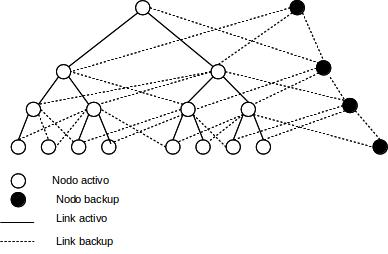
\includegraphics[scale=0.6]{images/binary_tree.jpg}
    	\end{column}
    	\begin{column}{.5\textwidth}
    		\begin{itemize}
    			\item Está compuesto por nodos y enlaces.
    			\item Está divididos en niveles. 
    			\item La FT de los árboles binarios vienen siendo estudiadas desde 1976.
    			\item Para lograr FT se las debe diseñar con un número mínimo de nodos de backup y link redundados. 
    		\end{itemize}
    	\end{column}
    \end{columns}
\end{frame}

\subsection{Redes Hypercube}
\begin{frame}
	\frametitle{Redes Hypercube}
	\begin{columns}[T]
		\begin{column}{.5\textwidth}
			% \centering
			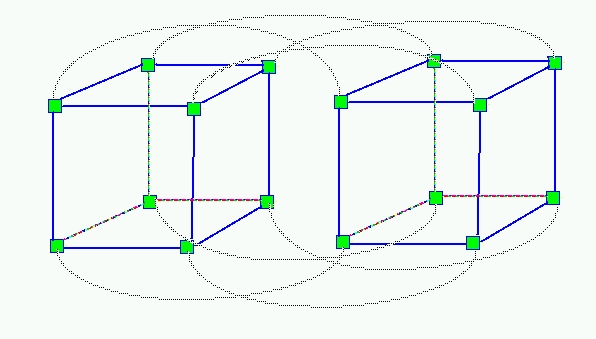
\includegraphics[scale=0.3]{images/cube.png}
		\end{column}
		\begin{column}{.5\textwidth}
			\begin{itemize}
				\item Tiene FT  de un componente. Si se produce una falla, no se transmite a todo el sistema. 
				\item Disponibilidad de enlaces entre cualquier par de nodos. 
				\item Existe una gran cantidad de enlaces. Esto aplicado en el ambiente espacial representa un problema. 
				
			\end{itemize}
		\end{column}
	\end{columns}
\end{frame}

\subsection{Redes distribuidas}
\begin{frame}
	\frametitle{Redes distribuidas}
	\begin{columns}[T]
		\begin{column}{.5\textwidth}
			% \centering
			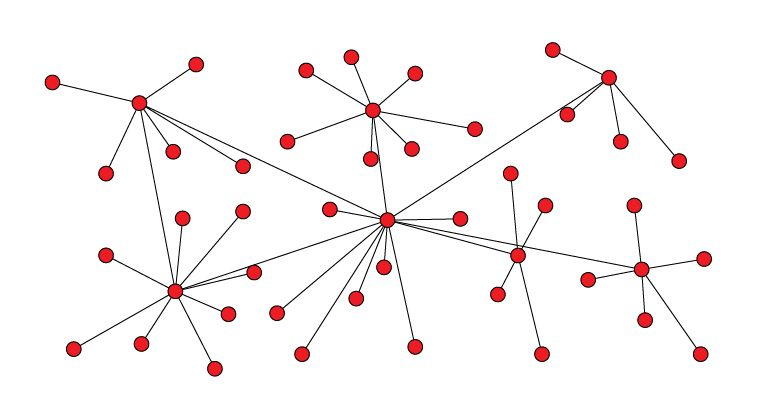
\includegraphics[scale=0.25]{images/distribuida.png}
		\end{column}
		\begin{column}{.5\textwidth}
			\begin{itemize}
				\item Red de nodos que se encuentran interconectados, intercambian información. 
				\item No existe un nodo central que gestione la red. 
				\item Una red distribuida es tolerante a fallas si puede formar subredes.
				\item Son necesarios el desarrollo y/o utilización de algoritmos de ruteo.
			\end{itemize}
		\end{column}
	\end{columns}
\end{frame}

\subsection{Redes TTEthernet en aviónica}
\begin{frame}
	\frametitle{Redes TTEthernet en aviónica}
	\begin{columns}[T]
		\begin{column}{.5\textwidth}
			% \centering
			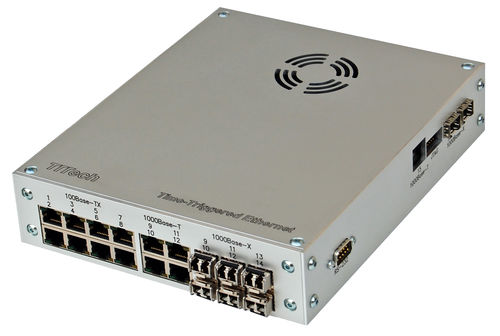
\includegraphics[scale=0.4]{images/ttethernet.png}
		\end{column}
		\begin{column}{.5\textwidth}
			\begin{itemize}
				\item TTEthernet es una tecnología basada en ethernet clásico. 
				\item Estandarizada como SAE AS6802.
				\item Transmite datos 100 veces más rápido que la que lo hacen las tecnologías tradicionales como el MIL-STD-1553.
				\item Fue utilizado en misiones como el Space Shuttle y la Estación Espacial Internacional (ISS).
				\item No cumple con el determinismo  requerido. 
			\end{itemize}
		\end{column}
	\end{columns}
\end{frame}